\section{Bivariate Plots in R}


Let's use a dataset called |iris|, that is included in the standard R distribution, to explore bivariate relationships between variables. This data set was made famous by R. A. Fisher who used it to illustrate many of the fundamental statistical methods he developed. The data set consists of four morphometric measurements for specimens from three different iris species. Use the R help to read about the iris data set (\lstinline!?iris!). We'll be using this data set repeatedly in future weeks so familiarize yourself with it.
%
\begin{R}
> ?iris
> names(iris)
[1] "Sepal.Length" "Sepal.Width"  "Petal.Length" "Petal.Width"
[5] "Species"
> unique(iris$Species)
[1] setosa     versicolor virginica
Levels: setosa versicolor virginica
> dim(iris)
[1] 150   5
\end{R}

For now let's just work with the \Species{I.~setosa} specimens. Read the help file for |subset()|.
\begin{R}
> setosa <- subset(iris, Species == 'setosa', select = -Species)
> dim(setosa)
[1] 50  4
> names(setosa)
[1] "Sepal.Length" "Sepal.Width"  "Petal.Length" "Petal.Width"
\end{R}
Notice how we used the |select| argument to |subset()| in order to drop the Species column. Let's explore the setosa subset with some graphs.
%
\begin{R}
> plot(setosa$Sepal.Length, setosa$Sepal.Width)
> plot(setosa$Sepal.Width ~ setosa$Sepal.Length)
\end{R}
Did you notice what is different between the two versions above? You can
also use the \lstinline!data! argument with plot, like so:
\begin{R}
> plot(Sepal.Width ~ Sepal.Length, data = setosa)
\end{R}
The \lstinline!xyplot()! function from the \lstinline!lattice! package
does pretty much the same thing:
%
\begin{R}
> library(lattice)
> xyplot(Sepal.Width ~ Sepal.Length, data = setosa)
\end{R}

Let's also explore a number of the other bivariate relationships in this data set:
%
\begin{R}
# an alternate way to generate such a plot, using the data argument to specify where the variables are defined
> plot(Petal.Length ~ Sepal.Length, data = setosa)

# same form as the first plot, but changing the character used for the plot using the 'pch' argument. The 'cex' argument increases the size of the characters by the specified factor (1.5x in this case)
> plot(setosa$Sepal.Length, setosa$Petal.Width, pch = 20, cex=1.5)
\end{R}

Often times it's useful to look at many bivariate relationships simultaneously. The |pairs()| function allows you to do this:
%
\begin{R}
> pairs(setosa)
\end{R}
%
\begin{figure}[htbp]
\centering
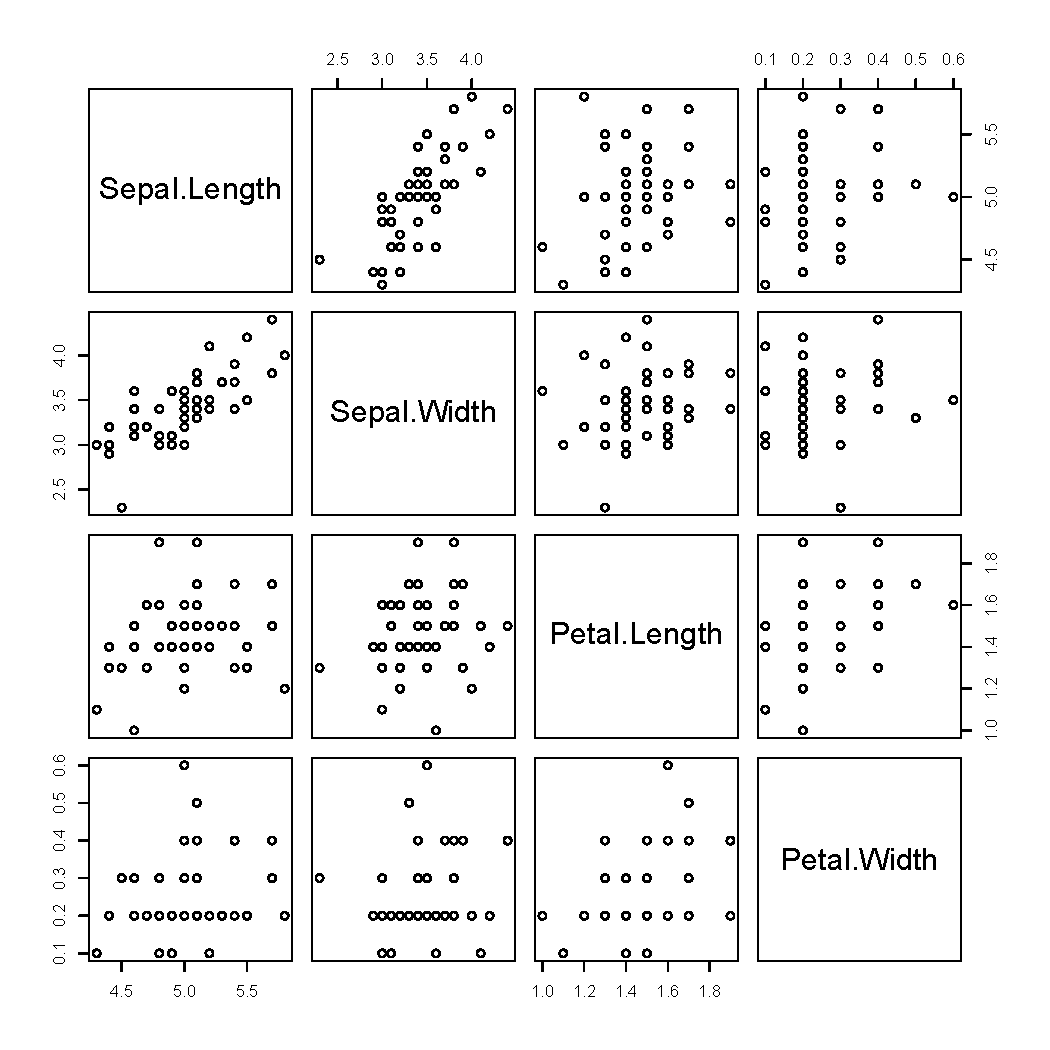
\includegraphics[width=0.5\columnwidth]{./figures/hands-on2/pairs-output.pdf}
\caption{Output of the \lstinline!pairs()! function for the \Species{I.~setosa} specimens in the \lstinline|iris| dataset.}
\end{figure}

Let's return to our use of the dot product to explore the relationship between variables. First let's add a function to |vecgeom.R| to calculate the cosine of the angle between to vectors.
\begin{R}
# add to vecgeom.R

vec.cos <- function(x,y,center=TRUE) {
  # Calculate the cos of the angle between vectors x and y
  if (center){
    x <- x-mean(x)
    y <- y-mean(y)
  }
  len.x <- veclength(x)
  len.y <- veclength(y)
  return( (x %*% y)/(len.x * len.y) )
}
\end{R}
We can then use this funciton to examine the relationship between the variables in the setosa dataset.
\begin{R}
> source("/Users/pmagwene/Downloads/vecgeom.R")
> vec.cos(setosa$Sepal.Length, setosa$Sepal.Width)
          [,1]
[1,] 0.7425467
> vec.cos(setosa$Sepal.Length, setosa$Petal.Length)
          [,1]
[1,] 0.2671758
> vec.cos(setosa$Sepal.Length, setosa$Petal.Width)
          [,1]
[1,] 0.2780984
\end{R}
Consider the values above in the context of the scatter plots you generated with the |pairs()| function; and then recall that for mean-centered variables, $\mathsf{cor}(X,Y) = r_{XY} = \cos \theta = \frac{\vec{x} \cdot \vec{y}}{\vert \vec{x}\vert \vert \vec{y} \vert}$.  So our |vec.cos()| function is equivalent to calculating the correlation between $x$ and $y$.  Let's confirm this using the built in |cor()| function in R:
\begin{R}
> cor(setosa$Sepal.Length, setosa$Sepal.Width)
[1] 0.7425467
> cor(setosa)  # called like this will calculate all pairwise correlations
             Sepal.Length Sepal.Width Petal.Length Petal.Width
Sepal.Length    1.0000000   0.7425467    0.2671758   0.2780984
Sepal.Width     0.7425467   1.0000000    0.1777000   0.2327520
Petal.Length    0.2671758   0.1777000    1.0000000   0.3316300
Petal.Width     0.2780984   0.2327520    0.3316300   1.0000000
\end{R}